
Utilizando como base \textcite{pesquisa}, pode-se dizer que a pesquisa adota
uma abordagem quantitativa e experimental, ou seja, visa analisar e contrastar o desempenho
de diferentes algoritmos em condições controladas. A natureza aplicada do estudo busca não
apenas compreender as nuances de cada algoritmo, mas também oferecer \textit{insights} para a seleção
e implementação dos mais eficazes. A metodologia descritiva permite uma análise detalhada
dos resultados obtidos, destacando as diferenças significativas entre os modelos avaliados.

\subsection{Solução proposta} \label{sec:solucao}

\begin{figure}[!htb] \centering
    \caption{Fluxo de implementação da solução} \label{figura:proposta}
    \begin{varwidth}{\linewidth}
      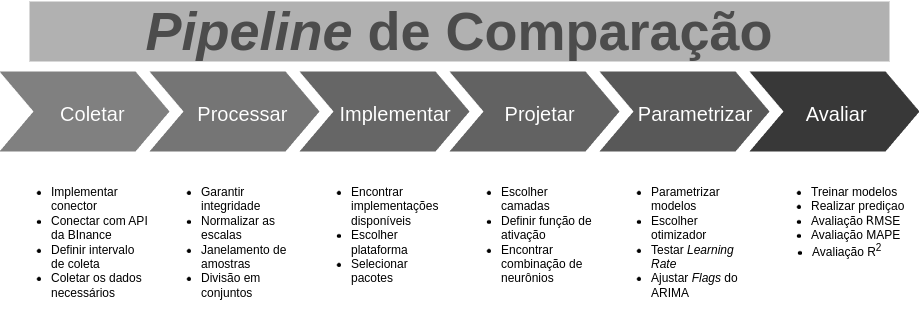
\includegraphics[width=16cm]{figuras/proposta.png}
      \fonte{Elaborado pelo autor, 2024.}
    \end{varwidth}
  \end{figure}

\section{Coleta de dados} \label{sec:coleta}
A coleta de dados ou obtenção de \textit{Datasets} envolve inicialmente selecionar locais como APIs, bancos de dados online ou arquivos históricos que forneçam os dados em um formato estruturado, como JSON, CSV ou TOML.
Mas, é possível estabelecer um processo de coleta automatizada através de \textit{Crawlers} ou \textit{Web Scrapping} para extrair as informações brutas.
Independente da escolha sempre é preciso realizar um projeto de dados, que envolve a definição de quais informações são relevantes e sua correlação, para isso, existem métodos como a análise exploratória de dados (EDA) e a visualização de dados como no \textit{Pair Plot}.
A tabela \ref{tab:amostras} apresenta um exemplo de amostras que foram coletadas.

\section{Pré processamento} \label{sec:preprocessamento}
No processo de análise de dados, é comum que os dados brutos apresentem inconsistências, como valores ausentes, duplicados ou mal formatados. 
Essas imperfeições comprometem a eficácia dos modelos, antes de enviar os dados para o treinamento, é crucial assegurar que estejam completos, formatados e escalonados de maneira adequada.
A essa etapa dá-se o nome de pré-processamento.

\begin{table}[!htb]
    \caption{Amostras da base de dados coletada} \label{tab:amostras}
    \begin{tabularx}{\textwidth}{X|X|X|X}
    \hline
    Data (GMT-3) & Volume & Trocas & Preço \\ \hline
    2020-01-01 00:00:00   & 1959651,83      & 2811            & 7228,5         \\ \hline
    2020-01-01 00:15:00   & 1225409,70      & 1897            & 7237,15        \\ \hline
    2020-01-01 00:30:00   & 1469869,68      & 2163            & 7221,27        \\ \hline
    2020-01-01 00:45:00   & 1012436,07      & 1466            & 7225,01        \\ \hline
    2020-01-01 01:00:00   & 1102372,81      & 1985            & 7219,09        \\ \hline
    \end{tabularx}
    \fonte{Elaborado pelo autor, 2024.}
\end{table}

\subsection{Validação de completude} \label{sec:completude}
Para verificar a completude dos dados, foi utilizada uma função nativa do \textit{Pandas}, garantindo que todas as entradas estejam presentes na base.
Embora o conector a realize na captura, é necessário uma verificação adicional a cada análise para assegurar a qualidade das amostras. 
Caso exista valores ausentes, é possível utilizar métodos como a interpolação para estimar os valores faltantes e preenchê-los.

\subsection{Normalização} \label{sec:normalizar}
Em um \textit{Dataset} multivariado é comum que os valores estejam em escalas distintas, no caso do \textit{Bitcoin}, o preço e o volume variam em ordens de grandeza superiores ao número absoluto de transações.
Isso se deve à própria natureza da dimensão dos dados, por isso, é necessário padronizar as variáveis para que o modelo não seja enviesado.
Uma das técnicas de normalização mais famosas ajusta as colunas para um intervalo que esteja entre o máximo e o mínimo valor encontrado, assim,  é chamada de \textit{MinMaxScaller}.
\begin{equation}
    {X_{Scalled} = \frac{X-X_{min}}{X_{max}-X_{min}}}
    \label{eq:scalled}
\end{equation}

Na equação acima, x é o valor original da variável, min(x) é o valor mínimo encontrado na coluna e max(x) o valor máximo.
Ao final obtemos o equivalente dimensionado da respectiva linha, ajustado em escala de 0 a 1.

\subsection{Limitações e diferenças entre algoritmos} \label{sec:limitacao}
O processamento de dados em diferentes algoritmos, seja no aprendizado de máquina ou modelagem estatística, requer um dimensionamento de dados contendente com as necessidades e limitações de cada método.
Ao utilizar redes neurais, é comum que o modelo consiga lidar bem com múltiplas variáveis e forneça um arcabouço robusto de soluções adquiridas durante o treinamento.

Por outro lado, modelos como a regressão linear são tradicionalmente univariados, significando que modelam uma única variável de interesse.
Outra característica é que não são treinados no sentido tradicional, em vez disso, ajustam seus parâmetros diretamente aos valores históricos, requerendo dados estacionários.
Ou seja, as entradas devem ser ligeiramente adaptadas às necessidades do modelo.

\subsection{Janelamento} \label{sec:janelamento}

Ao se trabalhar com séries temporais é comum a separação dos dados em segmentos menores
 a fim de capturar a dinâmica ao longo do tempo.
Uma dessas técnicas envolve a criação de janelas deslizantes, na qual um intervalo fixo de observações é utilizado para prever os próximos valores.
No contexto de redes neurais, essa abordagem é bastante útil, pois permite que o modelo capture padrões locais e evolutivos, aproveitando o poder da memória da rede para entender sequências.

Entretanto, quando se trata de modelos estatísticos, o processo de segmentação é geralmente feito de maneira incremental.
Em vez de usar uma janela deslizante de tamanho fixo, o modelo pode se beneficiar de uma janela expansiva, onde todos os dados disponíveis até um determinado ponto são utilizados para fazer a previsão seguinte.
Isso torna justa a comparação, visto que o máximo de informação disponível é utilizada para cada previsão.

\begin{figure}[!htb] \centering
    \caption{Técnicas de janelamento} \label{figura:window}
    \begin{varwidth}{\linewidth}
      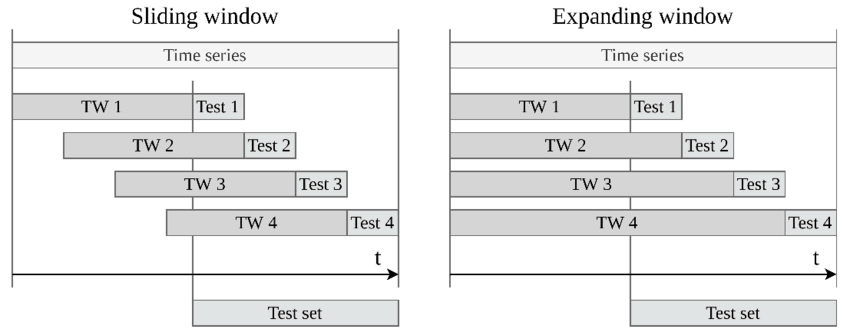
\includegraphics[width=12cm]{figuras/window.png}
      \fonte{\citefonte{Sliding}.}
    \end{varwidth}
\end{figure}
  

\subsection{Divisão em conjuntos} \label{sec:divisao}
Para avaliar a eficácia dos modelos de aprendizado supervisionado, a base de dados é dividida em três subconjuntos: treinamento, validação e teste.
O conjunto de treinamento é usado para ajustar os pesos do modelo, enquanto o de validação serve para otimizar os hiperparâmetros com base na função de perda.
Após o limite de épocas o conjunto de teste, que contém dados que o modelo ainda não viu, é utilizado para verificar a capacidade de generalizar seu desempenho. A etapa não é necessária para o ARIMA, que ajusta seus parâmetros diretamente sobre todos os dados.

\begin{figure}[!htb] \centering
    \caption{Divisão de dados} \label{figura:train_test}
    \begin{varwidth}{\linewidth}
      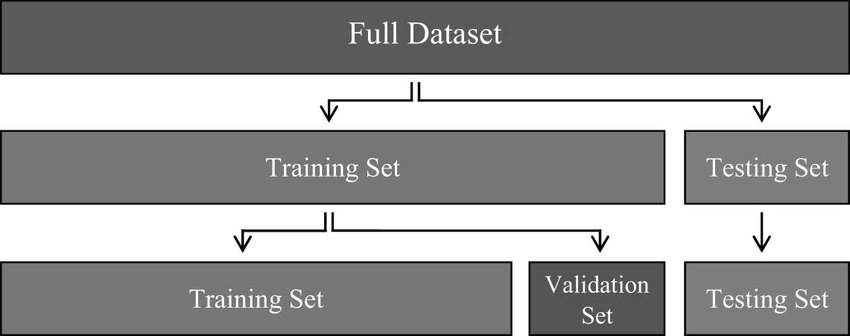
\includegraphics[width=12cm]{figuras/train_test.png}
      \fonte{\citefonte{Sliding}.}
    \end{varwidth}
\end{figure}

\section{Implementação} \label{sec:implementacao}
Todos os modelos foram desenvolvidos utilizando a linguagem de programação \textit{Python} versão 3.10 \cite{ramalho}, juntamente com as bibliotecas \textit{Pandas} e \textit{Numpy} \cite{Data}. 
Na implementação de redes neurais foram utilizados os \textit{Frameworks} Keras 3.10 e TensorFlow 2.10 \cite{maosaobra}, essas ferramentas podem ser adaptadas para processamento paralelo em GPU, mas, para isso a placa de video deve ter suporte a CUDA, tecnologia de codigo aberto da NVIDIA.
O ARIMA foi feito e otimizado com base no Pmdarima, biblioteca que implementa o modelo de forma eficiente.

\section{Arquitetura} \label{sec:arquitetura}
Para \textcite{Good} a arquitetura de uma rede define sua estrutura geral, incluindo o número de unidades e a forma como estão conectadas entre si
Cada modelo foi implementado de acordo com as especificações definidas para avaliação, respeitando as particularidades de cada um em relação à estrutura e aos parâmetros ajustados.
A seguir, são apresentadas as principais características os diferenciam e justificam seu desempenho nas análises.

\begin{table}[h!] \label{tabela:lstm_struct}
    \caption{Estrutura do modelo baseado em LSTM}
    \begin{tabularx}{\textwidth}{X|X|X|c|X} \hline
    Camada & Tipo & Neurônios & Função de Ativação & Parâmetros \\ \hline
    1 & LSTM                    & 32 & Tangente Hiperbólica                           & 4.000                  \\ \hline
    2 & Densa                   & 32 & Tangente Hiperbólica                            & 1.056                    \\ \hline
    3 & Densa                   & 1  & Linear                           & 33                     \\ \hline
    \end{tabularx}
    \fonte{Elaborado pelo autor, 2024.}
\end{table}

\begin{table}[h!] \label{tabela:gru_struct}
    \caption{Estrutura do modelo baseado em GRU}
    \begin{tabularx}{\textwidth}{X|X|X|c|X} \hline
    Camada & Tipo & Neurônios & Função de Ativação & Parâmetros \\ \hline
    1      & GRU  & 32  & Tangente Hiperbólica     & 3.552                 \\ \hline
    2      & Densa & 32 & Tangente Hiperbólica     & 1.056                    \\ \hline
    3      & Densa & 1  & Linear                   & 33                     \\ \hline
    \end{tabularx}
    \fonte{Elaborado pelo autor, 2024.}
\end{table}

\begin{table}[h!] \label{tabela:bidirectional_struct}
    \caption{Estrutura do modelo baseado em camadas Bidirecionais}
    \begin{tabularx}{\textwidth}{X|X|X|c|X} \hline
    Camada & Tipo & Neurônios & Função de Ativação & Parâmetros \\ \hline
    1                   & Bidirectional            & 32                   & Tangente Hiperbólica                         & 9.216                \\ \hline
    2                   & Densa                   &  32               & Tangente Hiperbólica                           & 2.000                 \\ \hline
    3                   & Densa                   &  1                   & Linear                       & 33                     \\ \hline
    \end{tabularx}
    \fonte{Elaborado pelo autor, 2024.}
\end{table}
    





\section{Configuração} \label{sec:configuracao} 
Os parâmetros da rede foram definidos de forma geral e aplicados uniformemente a todos os modelos avaliados. A configuração padrão adotada é descrita detalhadamente na Tabela \ref{tabela:parametros}.

\begin{table}[h!]
    \caption{Configuração dos parâmetros das redes neurais} \label{tabela:parametros}
    \begin{tabularx}{\textwidth}{X|X} \hline
    Parâmetros & Valores \\ \hline
    Batch         & 32               \\ \hline
    Épocas         & 500              \\ \hline
    Otimizador               & Nadam ($\eta=1*10^{-4}$; $\beta_1=0{,}85$; $\beta_2=0{,}989$; $\epsilon=10^{-6}$)             \\ \hline
    Fator de decaimento          & 0,5 em 20 épocas de platô            \\ \hline
    Função de perda          & MSE              \\ \hline
    \end{tabularx}
    \fonte{Elaborado pelo autor, 2024.}
\end{table}

\section{Avaliação} \label{sec:avaliacao}
Para avaliar a acurácia dos modelos de previsão, é preciso separar em duas categorias: aprendizado de máquina e estatística.
No aprendizado de máquina (supervisionado) é possivel validar diretamente na função de perda, que no caso é a MSE, enquanto nos estatísticos o cálculo é inerente à fórmula.

Na comparação final será feita uma combinação de métricas estatísticas 
que permitem analisar tanto a precisão quanto a robustez das previsões.
As métricas escolhidas para essa avaliação são: 
\textit{Mean Squared Error} (MSE), \textit{Root Mean Squared Error} (RMSE), \textit{Mean Absolute Percentage Error (MAPE)} e o Coeficiente de Determinação (R²). Cada uma dessas métricas fornece uma perspectiva única sobre a qualidade das previsões e será descrita a seguir.

\begin{equation}
    \text{MSE} = \frac{1}{n} \sum_{t=1}^{n} (\hat{y}_t - y_t)^2
\end{equation}

Calcula a média dos quadrados da diferença entre os valores previstos ŷ e os valores reais y. Penaliza erros maiores mais severamente, já que a diferenças é elevada ao quadrado

\begin{equation}
    \text{RMSE} = \sqrt{\frac{1}{n} \sum_{t=1}^{n} (y_t - \hat{y}_t)^2}
\end{equation}

A principal função dessa métrica é medir a diferença entre os valores observados 
y e os valores preditos $\hat{y}$, elevando o erro ao quadrado antes de calcular a média e aplicando a raiz quadrada ao final para que o erro tenha a mesma unidade dos dados originais. Isso significa que o RMSE dá maior peso a erros maiores devido ao efeito do quadrado,

\begin{equation}
    \text{MAPE} = \frac{1}{n} \sum_{t=1}^{n} \left|\frac{y_t - \hat{y}_t}{y_t}\right|
\end{equation}

Média dos erros percentuais absolutos na série, padronizando a análise para que seja possível comparar diferentes escalas ou unidades.
Quando a diferença entre y e ŷ é dividida por y, obtêm-se o percentual, que é então normalizado pela média. Como o somatório de valores decimais pode ser confuso, alguns autores sugerem multiplicar cada resultado por 100 para facilitar a interpretação.

\begin{equation}
    R^2 = 1 - \frac{\sum_{t=1}^{n} (y_t - \hat{y}_t)^2}{\sum_{t=1}^{n}(y_t - \bar{y})^2}
\end{equation}

O erro $R^2$, também chamado de coeficiente de determinação, representa a proporção da variabilidade dos dados que é explicada pelo modelo, variando de 0 a 1, sendo 1 o ajuste perfeito.
O $y_t$ define os valores reais, $\hat{y}_t$ os valores preditos e $\bar{y}$ é a média dos valores observados. O numerador contém a soma dos erros ao quadrado entre os valores reais e preditos (erro do modelo), enquanto o denominador é a soma da variabilidade total dos dados

\section{Materiais e Tecnologias} \label{sec:materiais}
Para a realização deste trabalho, 
foram utilizados um processador Intel Core i5-12500H e
uma placa de vídeo NVIDIA GeForce RTX 3050 de 4GB com suporte a CUDA 12
Um total de 16GB de memória RAM foram utilizados para armazenas os tensores, parâmetros e janelamento em memória dos dados. 
O sistema operacional foi o Linux Pop! OS 20.04 e o desenvolvimento foi feito no editor Visual Studio Code, utilizando Python 3.10. As bibliotecas empregadas incluíram Pandas e Numpy para manipulação e computação de dados, e Matplotlib e Seaborn para visualização. Para aprendizado de máquina e redes neurais, foram utilizados os frameworks Keras e TensorFlow, e o modelo ARIMA foi implementado com a biblioteca Pmdarima.